\documentclass{zjureport}
% \special{dvipdfmx:config z 0} % 调试时可关闭 PDF 压缩；最终提交保持注释

\usepackage{longtable}
\usepackage{hyperref}
\hypersetup{colorlinks=true, linkcolor=black, urlcolor=black, citecolor=black}
\providecommand{\tightlist}{%
  \setlength{\itemsep}{0pt}\setlength{\parskip}{0pt}}
\renewcommand\thesubsection{\arabic{section}.\arabic{subsection}}

% =============================================
% 报告信息
% =============================================

\major{电子科学与技术}
\name{金大钧}
\title{本科实验报告}
\stuid{3230103274}
\college{信息与电子工程学院}
\date{2026年6月24日}
\course{量子信息基础}
\instructor{钱浩亮}
\expname{双比特量子纠缠制备与 CHSH 不等式违背的蒙特卡洛验证}
\renewcommand{\figurename}{图}
\renewcommand{\tablename}{表}
\renewcommand{\refname}{参考文献}

\begin{document}

\makecover
\makecontent

\section*{摘要}
\addcontentsline{toc}{section}{摘要}

本项目以双比特 Bell 态为对象，利用量子态模拟和 Monte Carlo 抽样验证 CHSH 不等式的违背。仿真采用逐 shot 投影测量：每次重新制备纠缠态，按给定测量角依次测量 Alice 和 Bob，并由有限 shots 计数估计关联期望值 \(E\) 和 CHSH 参数 \(S\)。结果表明，在合适测量角下，\(|\Phi^+\rangle\) 的模拟结果满足 \(|S|>2\)，并接近量子理论值 \(2\sqrt{2}\)。项目还比较了四个 Bell 态的关联结构，并通过角度扫描和 visibility 噪声模型分析 CHSH 违背的影响因素。

\section{引言}\label{ux5f15ux8a00}

\subsection{研究背景}\label{ux7814ux7a76ux80ccux666f}

量子纠缠是量子信息中的基本现象。对于双粒子纠缠态，单个粒子的测量结果仍具有随机性，但两个粒子的联合测量结果可以表现出强关联。EPR 佯谬指出，这种远距离关联与经典定域实在论难以协调：如果物理量在测量前已有确定值，且远处测量选择不能影响本地结果，那么纠缠关联应当能够由局域隐变量解释。

Bell 不等式将这一问题转化为可检验的统计判据。若实验关联满足 Bell 不等式，局域隐变量模型仍可能成立；若实验关联违反 Bell 不等式，则说明经典定域模型无法解释该系统的统计结果。CHSH 不等式是 Bell 不等式最常用的双粒子二值测量形式。

\subsection{实验目标}\label{ux5b9eux9a8cux76eeux6807}

本实验围绕 CHSH 验证展开，主要目标如下：

\begin{enumerate}
\def\labelenumi{\arabic{enumi}.}
\item
  制备四种双比特 Bell 态。
\item
  在不同测量基下模拟有限 shots 重复测量。
\item
  由测量计数估计关联期望值 \(E\)，并计算 CHSH 参数 \(S\)。
\item
  验证合适测量角下的量子结果满足
\end{enumerate}

\[
|S|>2,
\]

并接近最大量子值

\[
|S|=2\sqrt{2}.
\]

\begin{enumerate}
\def\labelenumi{\arabic{enumi}.}
\setcounter{enumi}{4}
\tightlist
\item
  通过角度扫描、不同 Bell 态比较和噪声模型，分析 CHSH 违背的影响因素。
\end{enumerate}

\section{CHSH 实验原理}\label{chsh-ux5b9eux9a8cux539fux7406}

\subsection{实验设置}\label{ux5b9eux9a8cux8bbeux7f6e}

CHSH 实验包含两个测量方 Alice 和 Bob。一对粒子分别发送给两端，Alice 可选择测量设置 \(a\) 或 \(a'\)，Bob 可选择测量设置 \(b\) 或 \(b'\)。每次实验中，两端各选择一个设置并得到二值结果：

\[
A\in\{+1,-1\},\quad B\in\{+1,-1\}.
\]

大量重复实验后，可以分别统计四组测量设置

\[
(a,b),\quad (a,b'),\quad (a',b),\quad (a',b')
\]

下的联合结果分布，并由此计算统计关联。

\subsection{\texorpdfstring{关联函数 \(E\)}{关联函数 E}}\label{ux5173ux8054ux51fdux6570-e}

对测量设置 \((x,y)\)，其中 \(x\in\{a,a'\}\)，\(y\in\{b,b'\}\)，四种联合结果概率记为

\[
P_{++},\quad P_{+-},\quad P_{-+},\quad P_{--}.
\]

关联函数定义为

\[
E(x,y)=P_{++}+P_{--}-P_{+-}-P_{-+}.
\]

等价地，若将两端结果相乘，则

\[
E(x,y)=\langle AB\rangle.
\]

因此，\(E=1\) 表示完全正相关，\(E=-1\) 表示完全反相关，\(E=0\) 表示没有净相关。

\subsection{\texorpdfstring{CHSH 参数 \(S\)}{CHSH 参数 S}}\label{chsh-ux53c2ux6570-s}

CHSH 参数定义为

\[
S=E(a,b)+E(a,b')+E(a',b)-E(a',b').
\]

单个关联函数的取值范围为 \([-1,1]\)，不足以区分经典关联和量子纠缠关联。CHSH 判据的关键在于：对任何定域隐变量模型，上述四项组合必须满足

\[
|S|\leq 2.
\]

若实验得到

\[
|S|>2,
\]

则该统计结果不能由定域隐变量模型解释。

\subsection{经典上界的推导}\label{ux7ecfux5178ux4e0aux754cux7684ux63a8ux5bfc}

设每对粒子携带隐变量 \(\lambda\)。在定域隐变量理论中，Alice 的结果只依赖本地设置和 \(\lambda\)，Bob 的结果也只依赖本地设置和 \(\lambda\)。因此对固定的 \(\lambda\)，四个可能结果

\[
A(a,\lambda),\quad A(a',\lambda),\quad B(b,\lambda),\quad B(b',\lambda)
\]

均已确定，且只取 \(\pm1\)。

对固定 \(\lambda\)，CHSH 组合为

\[
S(\lambda)
=A(a,\lambda)B(b,\lambda)
+A(a,\lambda)B(b',\lambda)
+A(a',\lambda)B(b,\lambda)
-A(a',\lambda)B(b',\lambda).
\]

整理得

\[
S(\lambda)
=A(a,\lambda)\left[B(b,\lambda)+B(b',\lambda)\right]
+A(a',\lambda)\left[B(b,\lambda)-B(b',\lambda)\right].
\]

由于 \(B(b,\lambda),B(b',\lambda)\in\{+1,-1\}\)，两个括号中一个为 \(0\)，另一个为 \(\pm2\)。于是

\[
|S(\lambda)|=2.
\]

实验观测值是对隐变量分布 \(\rho(\lambda)\) 的平均：

\[
S=\int \rho(\lambda)S(\lambda)\,d\lambda.
\]

因此

\[
|S|
=\left|\int \rho(\lambda)S(\lambda)\,d\lambda\right|
\leq \int \rho(\lambda)|S(\lambda)|\,d\lambda
\leq 2.
\]

这就是 CHSH 不等式。它给出了所有定域隐变量模型共同满足的经典上界。

\subsection{量子力学预言}\label{ux91cfux5b50ux529bux5b66ux9884ux8a00}

量子力学允许纠缠态在合适测量设置下违反 CHSH 不等式。对于最大纠缠双比特态，CHSH 参数可达到

\[
|S|_{\max}=2\sqrt{2},
\]

该值称为 Tsirelson 上界。它高于经典上界 \(2\)，说明量子纠缠可以产生强于经典定域模型允许范围的统计关联。

\clearpage

\section{量子模型与测量约定}\label{ux91cfux5b50ux6a21ux578bux4e0eux6d4bux91cfux7ea6ux5b9a}

\subsection{Bell 态}\label{bell-ux6001}

双比特计算基取为

\[
|00\rangle,\quad |01\rangle,\quad |10\rangle,\quad |11\rangle.
\]

四个 Bell 态定义为

\[
|\Phi^\pm\rangle=\frac{|00\rangle\pm|11\rangle}{\sqrt{2}},
\]

\[
|\Psi^\pm\rangle=\frac{|01\rangle\pm|10\rangle}{\sqrt{2}}.
\]

主实验使用

\[
|\Phi^+\rangle=\frac{|00\rangle+|11\rangle}{\sqrt{2}}.
\]

在线路模型中，\(|\Phi^+\rangle\) 可由 \(|00\rangle\) 经 Hadamard 门和 CNOT 门制备：

\[
|00\rangle
\xrightarrow{H\otimes I}
\frac{|00\rangle+|10\rangle}{\sqrt{2}}
\xrightarrow{\mathrm{CNOT}}
\frac{|00\rangle+|11\rangle}{\sqrt{2}}.
\]

其余 Bell 态可由 \(|\Phi^+\rangle\) 施加局域 Pauli 门得到。

\subsection{偏振测量基}\label{ux504fux632fux6d4bux91cfux57fa}

本文采用偏振光子测量角约定。角度为 \(\theta\) 的测量基为

\[
|+_\theta\rangle=\cos\theta|0\rangle+\sin\theta|1\rangle,
\]

\[
|-_\theta\rangle=-\sin\theta|0\rangle+\cos\theta|1\rangle.
\]

该约定下，对 \(|\Phi^+\rangle\) 有

\[
E(\theta_A,\theta_B)=\cos[2(\theta_A-\theta_B)].
\]

因此最优 CHSH 角为

\[
a=0^\circ,\quad a'=45^\circ,\quad b=22.5^\circ,\quad b'=-22.5^\circ.
\]

此时

\[
S=2\sqrt{2}.
\]

这里的因子 \(2\) 来自偏振角表示，因此不能直接套用自旋 \(1/2\) 约定下的角度。

\subsection{visibility 噪声模型}\label{visibility-ux566aux58f0ux6a21ux578b}

为模拟态制备误差、退相干或混合态污染，本文采用 visibility 混合模型：

\[
\rho_v=v|\Phi^+\rangle\langle\Phi^+|+(1-v)\frac{I_4}{4},
\quad 0\leq v\leq1.
\]

完全混合态不贡献净关联，因此最优角度下有

\[
S(v)=2\sqrt{2}v.
\]

CHSH 违背条件为

\[
v>\frac{1}{\sqrt{2}}\approx0.707.
\]

\subsection{仿真中的测量约定}\label{ux4effux771fux4e2dux7684ux6d4bux91cfux7ea6ux5b9a}

每个 shot 对应一次独立实验。仿真中先重新制备双比特态 \(\rho\)，再按给定角度进行投影测量。

对单比特测量角 \(\theta\)，先定义单比特投影算符

\[
P_+(\theta)=|+_\theta\rangle\langle+_\theta|,
\quad
P_-(\theta)=|-_\theta\rangle\langle-_\theta|.
\]

由于 \(\rho\) 是双比特密度矩阵，实际测量时需要将单比特投影算符扩展到双比特空间。测量 Alice 时使用

\[
\Pi_r^A=P_r(\theta_A)\otimes I,
\]

测量 Bob 时使用

\[
\Pi_r^B=I\otimes P_r(\theta_B).
\]

若当前使用的双比特投影算符记为 \(\Pi_r\)，测量结果 \(r\in\{+,-\}\) 的概率由 Born rule 给出：

\[
p_r=\mathrm{Tr}(\Pi_r\rho).
\]

若得到结果 \(r\)，测量后的态更新为

\[
\rho'=\frac{\Pi_r\rho\Pi_r}{\mathrm{Tr}(\Pi_r\rho)}.
\]

本项目每个 shot 先测 Alice，再测 Bob，并记录联合结果。Alice 和 Bob 的投影算符作用在不同量子比特上，因此该计算顺序不改变联合测量的理论统计结果。

\clearpage

\section{程序实现}\label{ux7a0bux5e8fux5b9eux73b0}

\subsection{实现流程}\label{ux5b9eux73b0ux6d41ux7a0b}

程序使用 NumPy 完成双比特态模拟，主要步骤为：

\begin{enumerate}
\def\labelenumi{\arabic{enumi}.}
\item
  制备 Bell 态，并写成密度矩阵。
\item
  根据 visibility 加入白噪声混合。
\item
  对每组测量角执行逐 shot 投影测量。
\item
  由计数估计 \(E_{\mathrm{sim}}\)。
\item
  由 Born 概率计算 \(E_{\mathrm{theory}}\) 作为理论参考。
\item
  由四组 \(E\) 组合得到 \(S_{\mathrm{sim}}\) 和 \(S_{\mathrm{theory}}\)。
\end{enumerate}

核心计算位于 \texttt{src/chsh.py}，命令行入口和绘图位于 \texttt{src/main.py}。

\subsection{逐 shot 投影测量}\label{ux9010-shot-ux6295ux5f71ux6d4bux91cf}

对一组角度 \((\theta_A,\theta_B)\)，程序重复执行 \(N\) 次独立 shot。每次 shot 的流程为：

\begin{enumerate}
\def\labelenumi{\arabic{enumi}.}
\item
  复制当前待测密度矩阵。
\item
  构造 Alice 的投影算符 \(P_+^A,P_-^A\)，随机得到 Alice 结果。
\item
  按投影测量规则更新双比特态。
\item
  构造 Bob 的投影算符 \(P_+^B,P_-^B\)，随机得到 Bob 结果。
\item
  将联合结果计入 \(N_{++},N_{+-},N_{-+},N_{--}\)。
\end{enumerate}

有限 shots 下的关联函数估计为

\[
\hat{E}
=\frac{N_{++}+N_{--}-N_{+-}-N_{-+}}{N}.
\]

这一过程用于生成 \(E_{\mathrm{sim}}\)。理论值 \(E_{\mathrm{theory}}\) 仍由联合 Born 概率计算，不参与随机抽样。

\subsection{实验设计}\label{ux5b9eux9a8cux8bbeux8ba1}

本项目包含四类实验：

\begin{enumerate}
\def\labelenumi{\arabic{enumi}.}
\item
  默认 CHSH 实验：使用 \(|\Phi^+\rangle\) 和最优偏振角，验证 \(|S|>2\)。
\item
  shots 收敛实验：改变 shots 数，观察 \(\hat{S}\) 向理论值收敛。
\item
  角度扫描实验：固定 \(a=0^\circ,a'=45^\circ,b=\theta,b'=-\theta\)，扫描 \(\theta\)。
\item
  噪声扫描实验：扫描 visibility \(v\)，观察 CHSH 违背随噪声增强而消失。
\end{enumerate}

\clearpage

\section{实验结果与分析}\label{ux5b9eux9a8cux7ed3ux679cux4e0eux5206ux6790}

\subsection{默认 CHSH 实验}\label{ux9ed8ux8ba4-chsh-ux5b9eux9a8c}

默认实验使用 \(|\Phi^+\rangle\)、shots \(=10000\)，测量角为

\[
a=0^\circ,\quad a'=45^\circ,\quad b=22.5^\circ,\quad b'=-22.5^\circ.
\]

四组关联期望值如下：

\begin{longtable}[]{@{}lrrr@{}}
\toprule\noalign{}
测量组合 & \(E_{\mathrm{sim}}\) & \(E_{\mathrm{theory}}\) & 误差 \\
\midrule\noalign{}
\endhead
\bottomrule\noalign{}
\endlastfoot
\(E(a,b)\) & 0.710400 & 0.707107 & 0.003293 \\
\(E(a,b')\) & 0.704800 & 0.707107 & -0.002307 \\
\(E(a',b)\) & 0.723000 & 0.707107 & 0.015893 \\
\(E(a',b')\) & -0.704600 & -0.707107 & 0.002507 \\
\end{longtable}

由此得到

\[
S_{\mathrm{sim}}=2.842800,\quad
S_{\mathrm{theory}}=2.828427.
\]

模拟结果超过经典上界 \(2\)，并接近 \(2\sqrt{2}\)，说明 \(|\Phi^+\rangle\) 在该测量设置下违反 CHSH 不等式。

\subsection{shots 收敛实验}\label{shots-ux6536ux655bux5b9eux9a8c}

改变 shots 数得到以下结果：

\begin{longtable}[]{@{}rrrr@{}}
\toprule\noalign{}
shots & \(S_{\mathrm{sim}}\) & \(S_{\mathrm{theory}}\) & 误差 \\
\midrule\noalign{}
\endhead
\bottomrule\noalign{}
\endlastfoot
100 & 2.760000 & 2.828427 & -0.068427 \\
500 & 2.768000 & 2.828427 & -0.060427 \\
1000 & 2.894000 & 2.828427 & 0.065573 \\
5000 & 2.844400 & 2.828427 & 0.015973 \\
10000 & 2.815000 & 2.828427 & -0.013427 \\
50000 & 2.820640 & 2.828427 & -0.007787 \\
\end{longtable}

\begin{figure}[H]
\centering
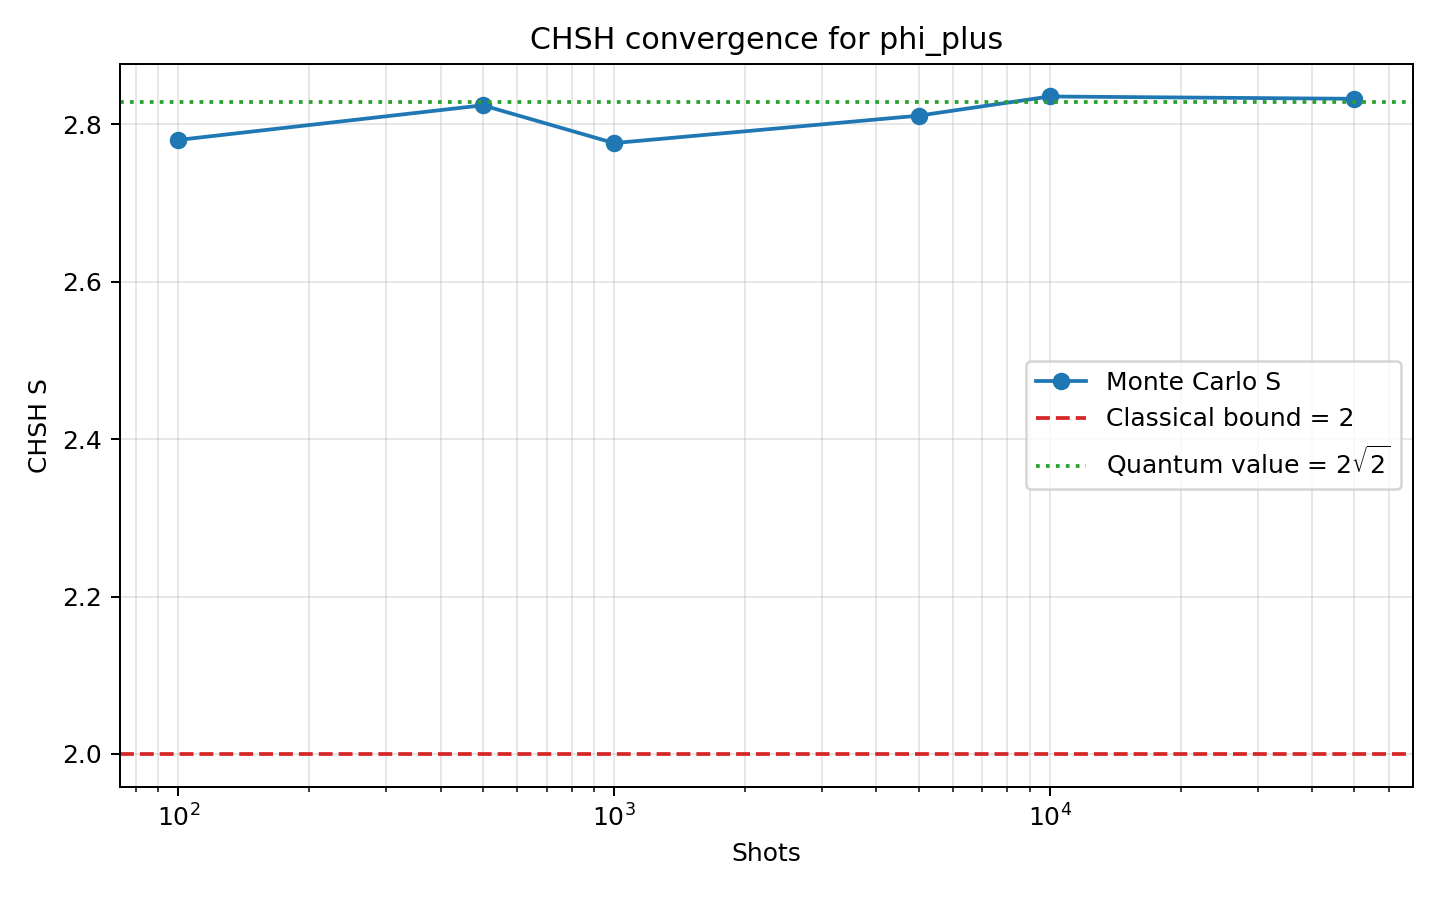
\includegraphics[width=0.82\linewidth]{../figures/chsh_mvp_convergence.png}
\caption{CHSH convergence}
\end{figure}

各 shots 设置下均有 \(S_{\mathrm{sim}}>2\)。需要注意，\(2\sqrt{2}\) 是无限重复测量下理论期望值的上界，而 \(S_{\mathrm{sim}}\) 是有限 shots 频率估计量。有限样本会使估计值围绕理论值波动，因此个别点可能略高于 \(2\sqrt{2}\)，例如 1000 shots 时的 \(S_{\mathrm{sim}}=2.894000\)。这不表示 Tsirelson 上界被突破；随着 shots 增加，结果应逐渐收敛到理论值附近。

\subsection{四个 Bell 态的比较}\label{ux56dbux4e2a-bell-ux6001ux7684ux6bd4ux8f83}

在同一组默认测量角下，四个 Bell 态的 CHSH 理论值不同。表中 \texttt{Phi+}、\texttt{Phi-}、\texttt{Psi+}、\texttt{Psi-} 分别表示 \(|\Phi^+\rangle\)、\(|\Phi^-\rangle\)、\(|\Psi^+\rangle\)、\(|\Psi^-\rangle\)。

\begin{longtable}[]{@{}lrl@{}}
\toprule\noalign{}
Bell 态 & 默认角度下的 \(S_{\mathrm{theory}}\) & 说明 \\
\midrule\noalign{}
\endhead
\bottomrule\noalign{}
\endlastfoot
Phi+ & 2.828427 & 与默认角匹配，正向最大违背 \\
Phi- & 0.000000 & 四项关联在该角度下抵消 \\
Psi+ & 0.000000 & 四项关联在该角度下抵消 \\
Psi- & -2.828427 & 绝对值最大，符号相反 \\
\end{longtable}

\(|\Phi^-\rangle\) 和 \(|\Psi^+\rangle\) 在默认角度下得到 \(S\approx0\)，说明该组测量角没有对准它们的 CHSH 违背方向。

\subsection{角度扫描实验}\label{ux89d2ux5ea6ux626bux63cfux5b9eux9a8c}

角度扫描固定

\[
a=0^\circ,\quad a'=45^\circ,\quad b=\theta,\quad b'=-\theta,
\]

并令 \(\theta\) 从 \(-45^\circ\) 扫描到 \(45^\circ\)。对 \(|\Phi^+\rangle\)，理论曲线在 \(\theta=22.5^\circ\) 附近达到最大值 \(2\sqrt{2}\)。本次 Monte Carlo 扫描中，最大模拟值出现在

\[
\theta=21.5^\circ,\quad S_{\mathrm{sim}}=2.865200.
\]

该值略高于 \(2\sqrt{2}\)，同样属于有限 shots 下的统计涨落。

\begin{figure}[H]
\centering
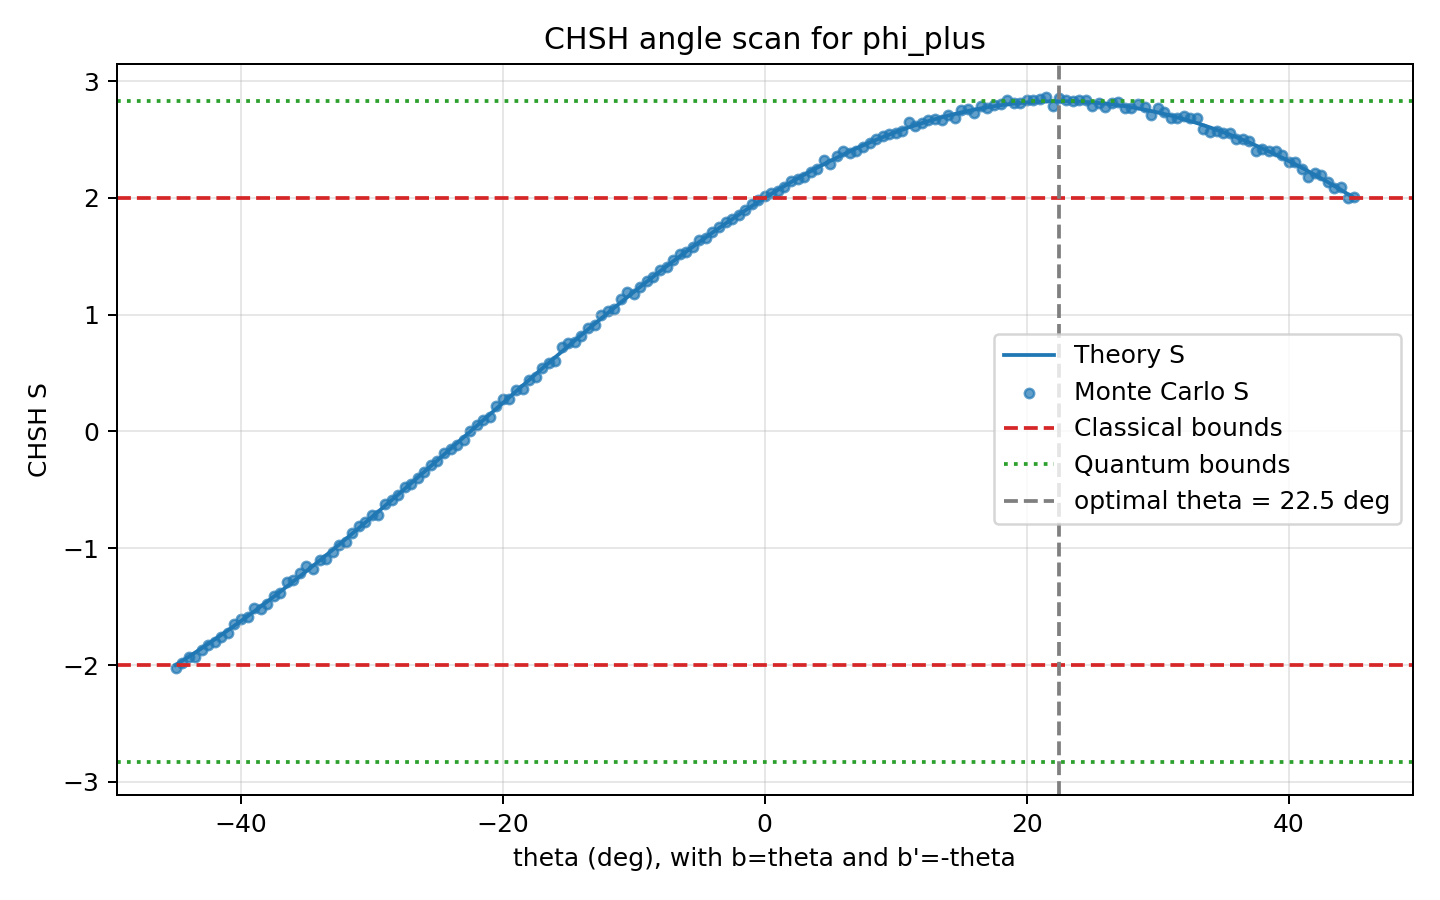
\includegraphics[width=0.82\linewidth]{../figures/phi_plus_angle_scan.png}
\caption{phi\_plus angle scan}
\end{figure}

\begin{figure}[H]
\centering
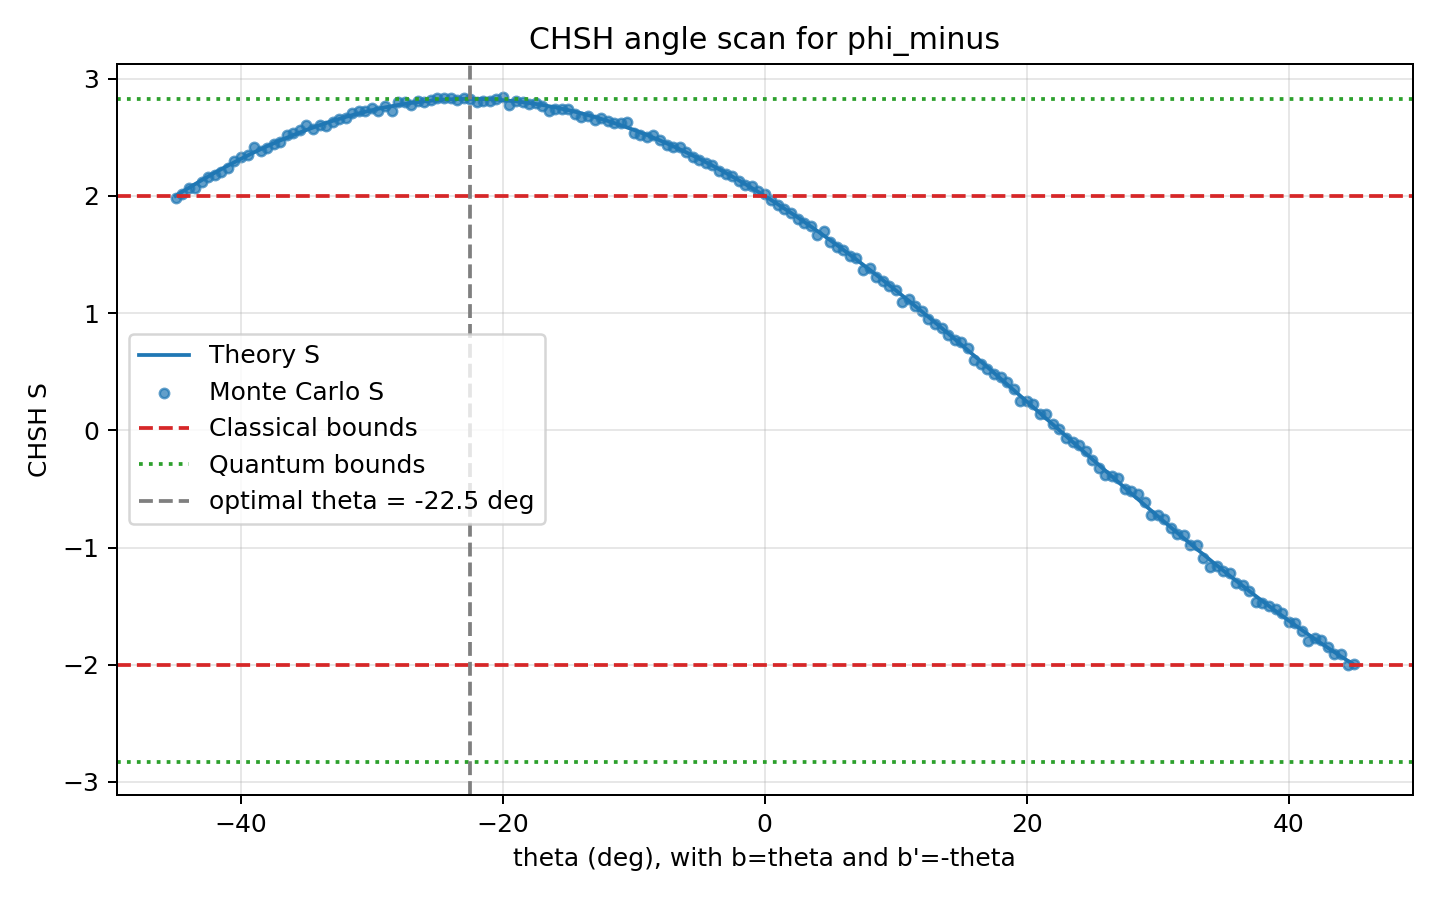
\includegraphics[width=0.82\linewidth]{../figures/phi_minus_angle_scan.png}
\caption{phi\_minus angle scan}
\end{figure}

\begin{figure}[H]
\centering
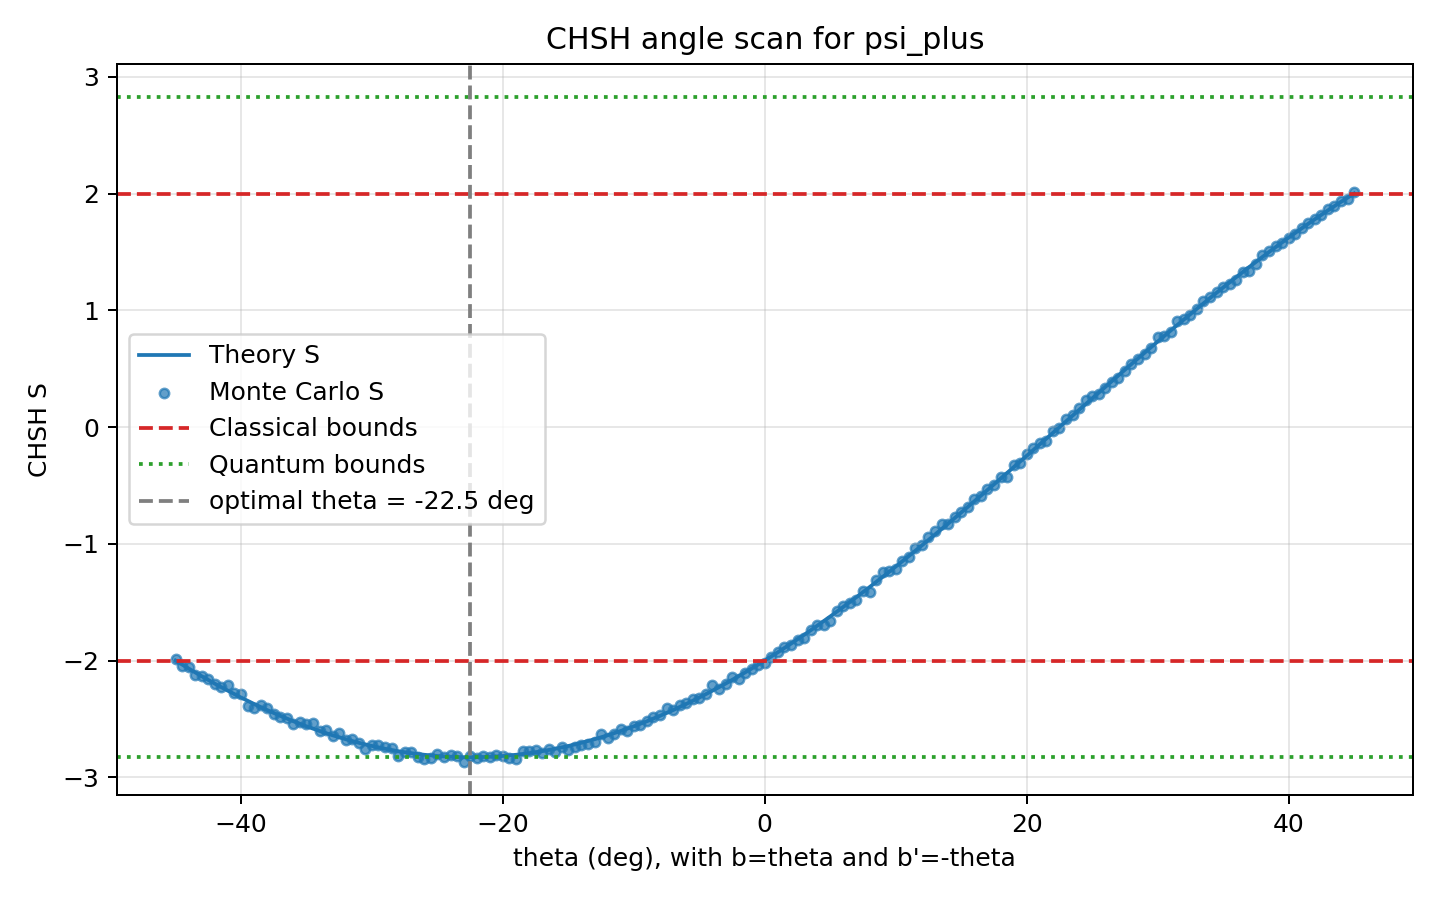
\includegraphics[width=0.82\linewidth]{../figures/psi_plus_angle_scan.png}
\caption{psi\_plus angle scan}
\end{figure}

\begin{figure}[H]
\centering
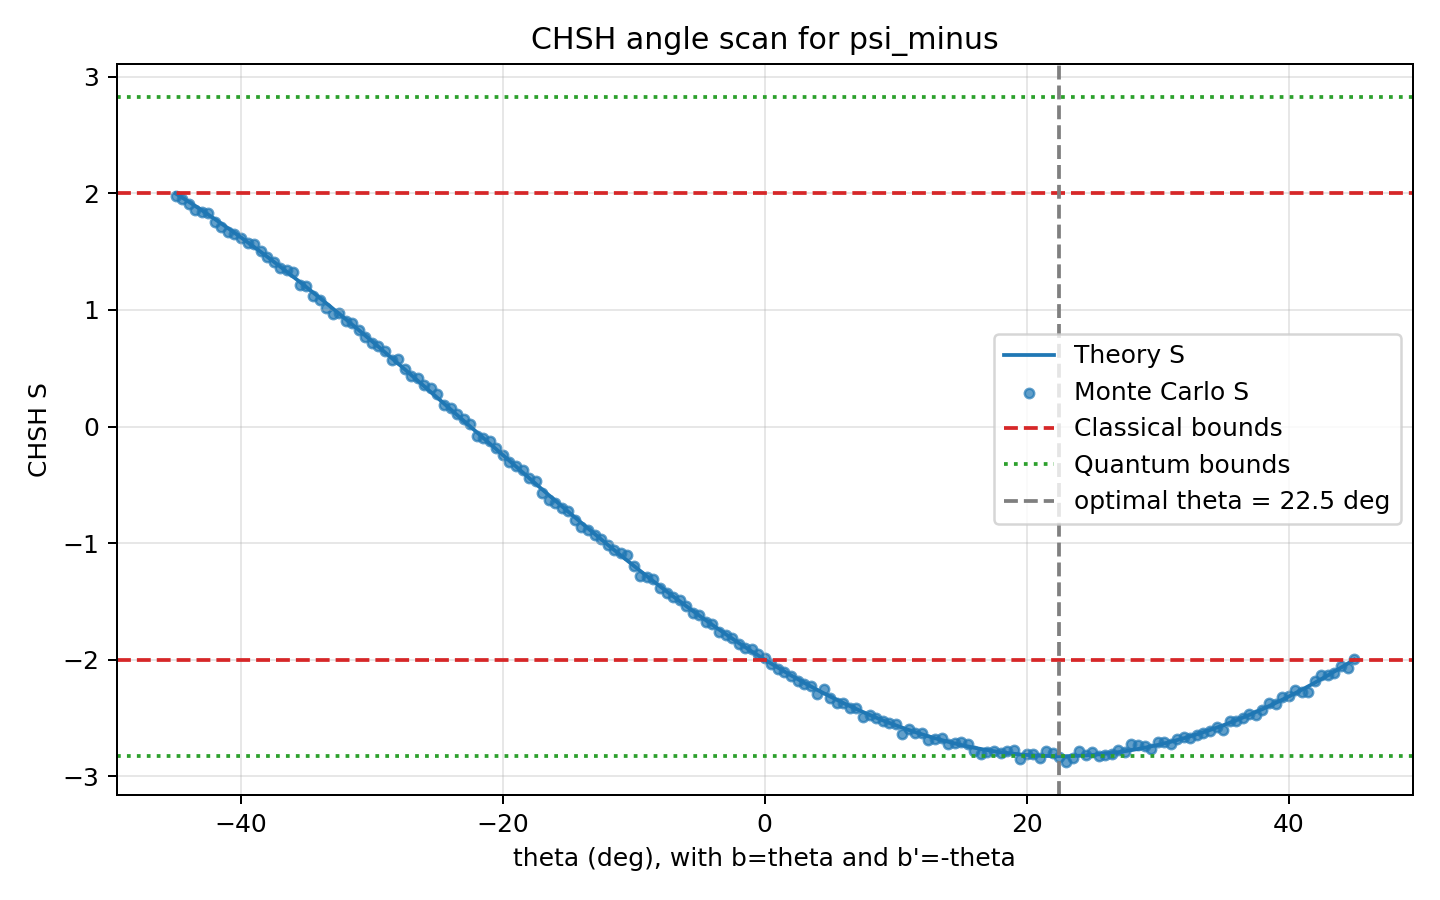
\includegraphics[width=0.82\linewidth]{../figures/psi_minus_angle_scan.png}
\caption{psi\_minus angle scan}
\end{figure}

扫描结果表明，不同 Bell 态的最优测量方向不同：\(|\Phi^+\rangle\) 在 \(\theta=22.5^\circ\) 附近取正向最大值，\(|\Psi^-\rangle\) 在同一方向取负向最大值；\(|\Phi^-\rangle\) 和 \(|\Psi^+\rangle\) 的最优方向位于 \(\theta=-22.5^\circ\) 附近。

\subsection{噪声扫描实验}\label{ux566aux58f0ux626bux63cfux5b9eux9a8c}

噪声扫描采用 visibility 模型。理论预测为

\[
S(v)=2\sqrt{2}v.
\]

临界附近结果如下：

\begin{longtable}[]{@{}rrr@{}}
\toprule\noalign{}
visibility \(v\) & \(S_{\mathrm{sim}}\) & \(S_{\mathrm{theory}}\) \\
\midrule\noalign{}
\endhead
\bottomrule\noalign{}
\endlastfoot
0.70 & 1.980400 & 1.979899 \\
0.71 & 1.997600 & 2.008183 \\
0.72 & 2.030000 & 2.036468 \\
1.00 & 2.797200 & 2.828427 \\
\end{longtable}

\begin{figure}[H]
\centering
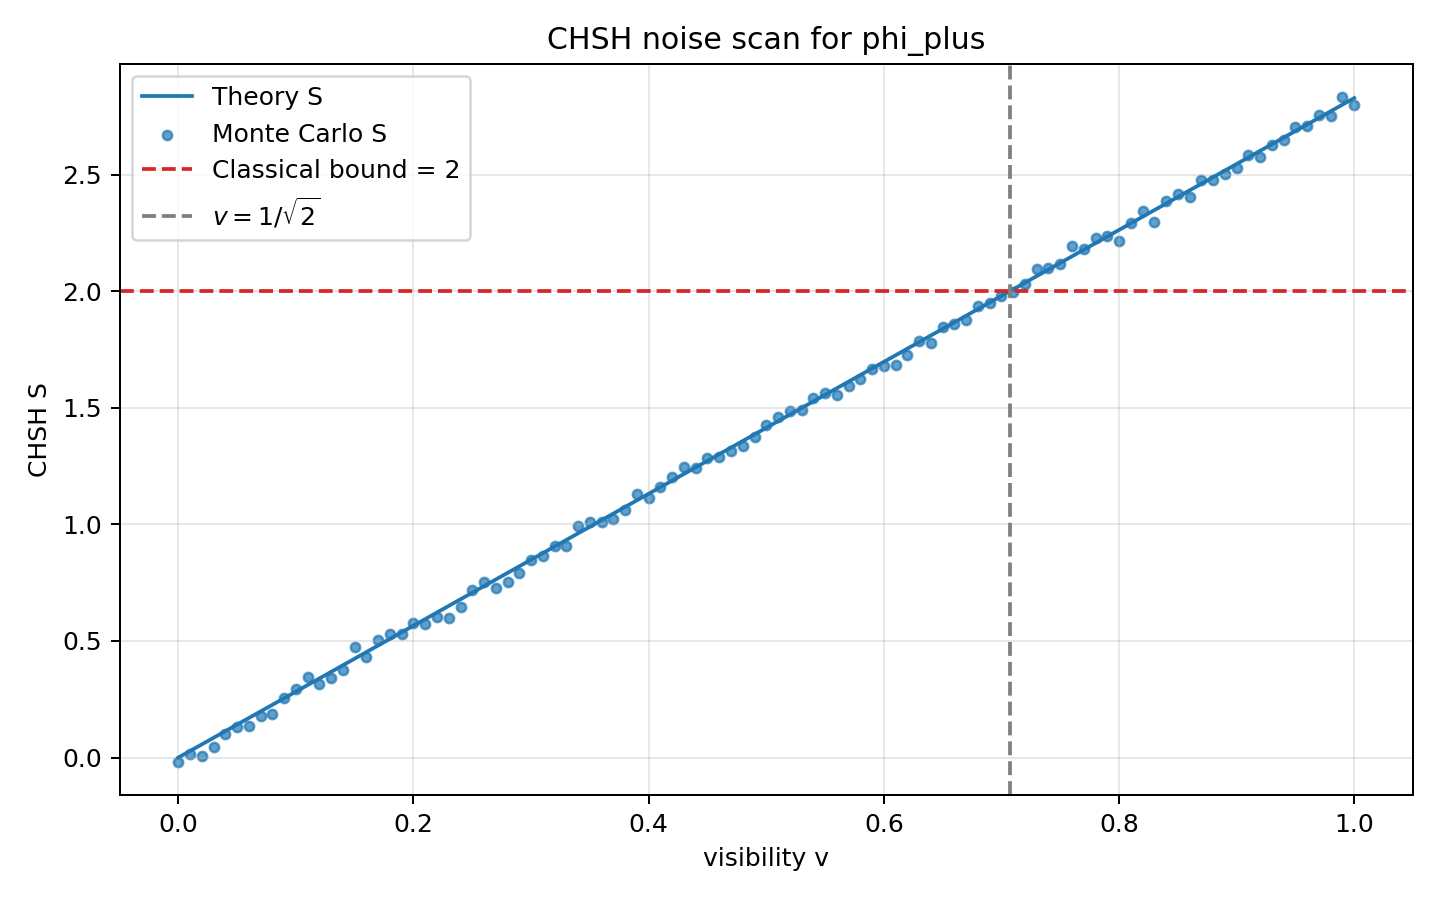
\includegraphics[width=0.82\linewidth]{../figures/chsh_noise_scan.png}
\caption{CHSH noise scan}
\end{figure}

理论临界值为

\[
v_c=\frac{1}{\sqrt{2}}\approx0.707.
\]

当 \(v>v_c\) 时，理论曲线超过经典上界 \(2\)；当 \(v<v_c\) 时，噪声使 CHSH 违背消失。Monte Carlo 点围绕理论线波动，符合有限 shots 的统计特征。

\clearpage

\section{仿真方法讨论}\label{ux4effux771fux65b9ux6cd5ux8ba8ux8bba}

\subsection{联合概率抽样方法的不足}\label{ux8054ux5408ux6982ux7387ux62bdux6837ux65b9ux6cd5ux7684ux4e0dux8db3}

项目早期实现采用联合概率抽样：先由密度矩阵和测量基计算

\[
P_{++},P_{+-},P_{-+},P_{--},
\]

再按该四项分布一次性抽取 \(N\) 次结果。该方法使用 Born rule，并非数学上错误；对理想投影测量而言，它与逐 shot 测量具有相同的联合分布。

但作为 CHSH 实验过程的主仿真，它的说服力不足。原因是它直接在联合结果层面抽样，没有显式体现每次实验中 Alice 和 Bob 的单次测量，也没有展示测量后的态更新。对于本课程大作业，``大量重复测量''的重点不仅是得到正确分布，也包括模拟实验中逐次制备、逐次测量、再统计关联的过程。

\subsection{逐 shot 投影测量方法的优势}\label{ux9010-shot-ux6295ux5f71ux6d4bux91cfux65b9ux6cd5ux7684ux4f18ux52bf}

当前实现改为逐 shot 投影测量。每个 shot 都重新制备态，先测 Alice，再根据测量结果更新态，随后测 Bob 并记录联合结果。该流程更接近 CHSH 实验叙事：

\[
\rho
\rightarrow
\text{Alice 测量}
\rightarrow
\rho'
\rightarrow
\text{Bob 测量}
\rightarrow
\text{联合结果}.
\]

这种方法避免直接从四个联合概率生成计数，改为通过单次测量概率和投影更新得到每个 shot 的结果。因此，\(E_{\mathrm{sim}}\) 更清楚地来自模拟测量计数，\(E_{\mathrm{theory}}\) 只作为理论对照。

\subsection{当前方法的局限性}\label{ux5f53ux524dux65b9ux6cd5ux7684ux5c40ux9650ux6027}

逐 shot 投影测量仍然不等同于真实物理实验。首先，它仍是经典计算机仿真，每次随机测量都需要由 Born rule 计算概率。其次，程序中 Alice 先测、Bob 后测是计算顺序；真实 CHSH 实验中，两端测量可以空间分离。由于两端投影算符作用在不同量子比特上，这一顺序不影响理想理论统计，但它仍是模拟假设。

此外，本项目未模拟探测器效率、暗计数、时间窗选择、测量基快速随机切换等实验细节。噪声部分也只采用简单 visibility 混合模型。因此，当前结果仍属于理想化模拟，不能视为对完整实验装置的复现。

\section{总结}\label{ux603bux7ed3}

本项目完成了 Bell 态制备、偏振基测量、逐 shot Monte Carlo 抽样、关联期望值统计和 CHSH 参数计算。默认 \(|\Phi^+\rangle\) 实验得到

\[
S_{\mathrm{sim}}=2.842800>2,
\]

验证了纠缠态对 CHSH 不等式的违背，并与理论值 \(2\sqrt{2}\) 符合较好。

进一步实验表明，CHSH 违背依赖测量基与 Bell 态关联结构的匹配关系；同一组测量角不能让所有 Bell 态同时达到最大违背。角度扫描展示了不同 Bell 态的最优测量方向，噪声扫描说明当 visibility 低于 \(1/\sqrt{2}\) 附近时，CHSH 违背会消失。

相比直接联合概率抽样，逐 shot 投影测量更清楚地体现了``制备---测量---统计''的实验过程。尽管该方法仍属于理想量子模拟，但已能较完整地展示 CHSH 不等式违背的主要物理机制和 Monte Carlo 验证过程。

\clearpage

\end{document}
